%!TeX root=main.tex
\section{Conclusions}\label{sec:conclusions}
%%%%%%%%%%%%%%%%%%%%%%%%%%%%%%%%%%%%%%%%%%%%%%%%%%%%%%%%
% HAD TO MOVE FIGURE FROM EXPERIMENTS HERE, OTHERWISE HALF OF A PAGE IS BLANK
%%%%%%%%%%%%%%%%%%%%%%%%%%%%%%%%%%%%%%%%%%%%%%%%%%%%%%%%%
\begin{figure}[t!]
	\vspace{-5mm}
	\centering
	\subfloat[Exposure loss for the non-protected group. \label{fig:experiments:compasAge:expGain:groupNP}]{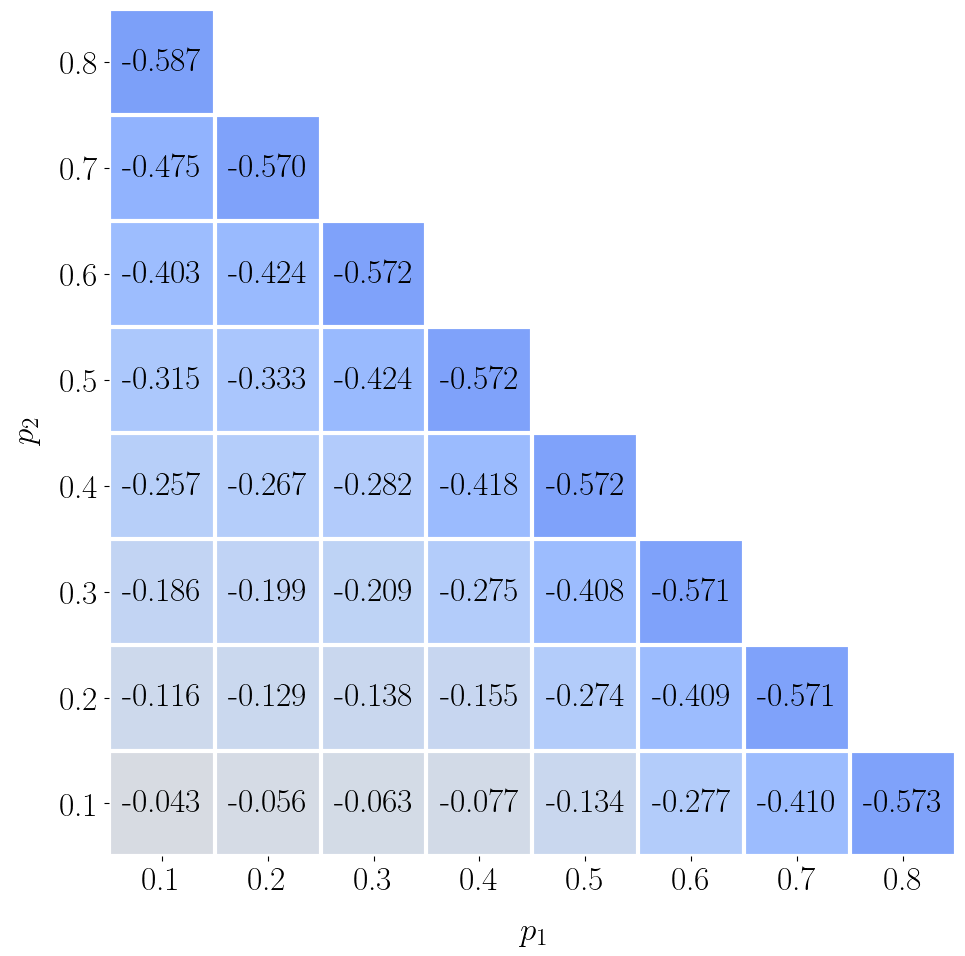
\includegraphics[width=.49\textwidth]{pics/k=200-heatmap-expGainGroupNP.png}}
	\subfloat[Exposure gain/loss for group ``age 25 -- 45''. \label{fig:experiments:compasAge:expGain:group1}]{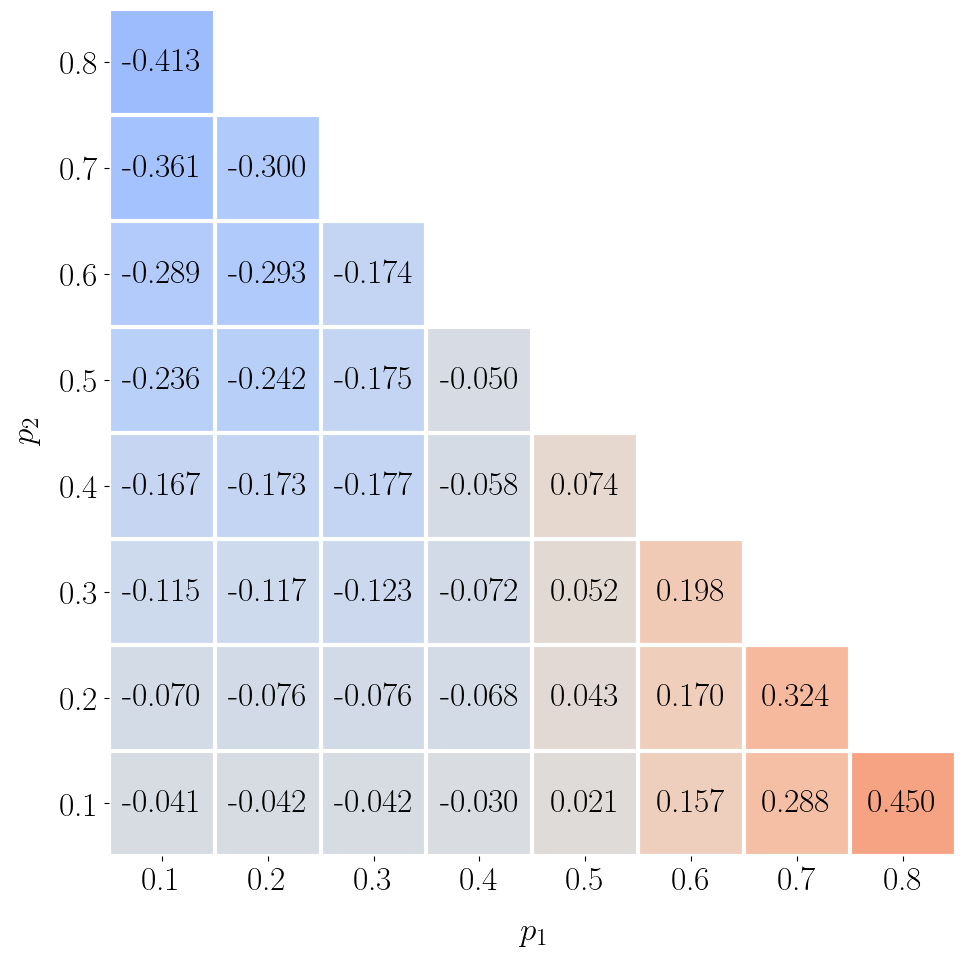
\includegraphics[width=.49\textwidth]{pics/k=200-heatmap-expGainGroup1.png}}\hfill
	\subfloat[Exposure gain for group ``age < 25''. \label{fig:experiments:compasAge:expGain:group2}]{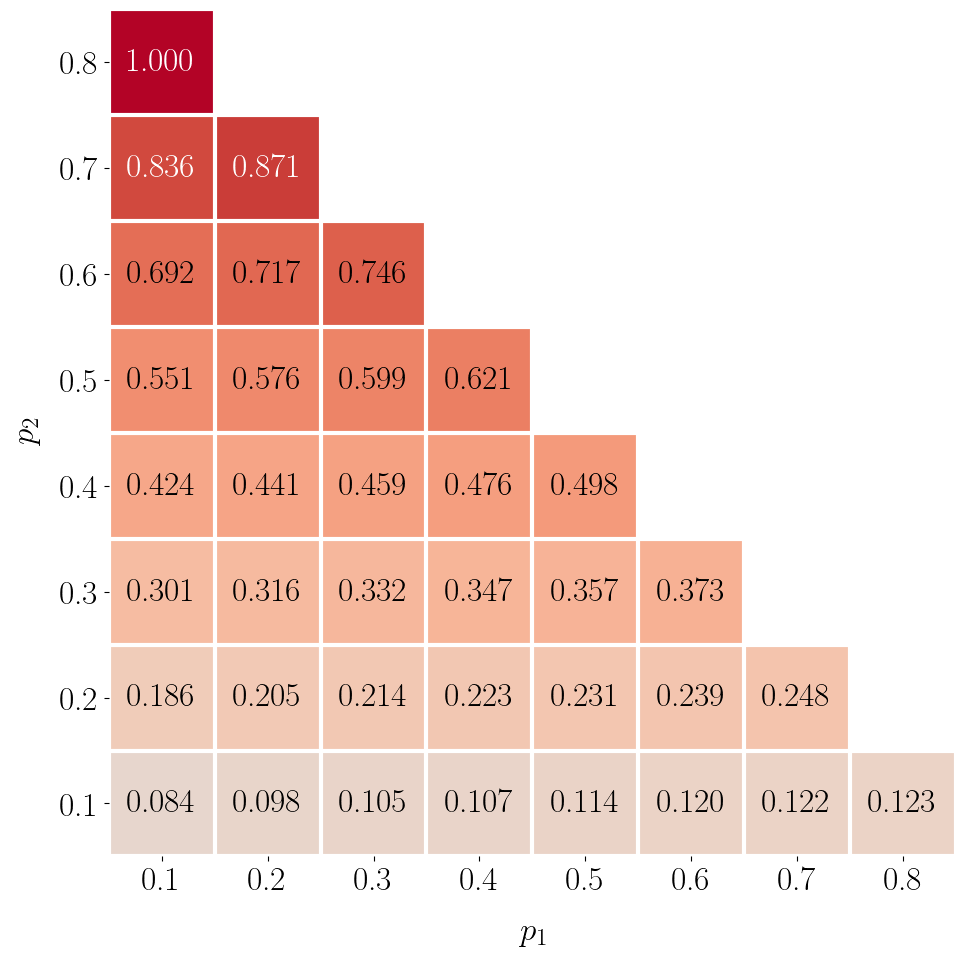
\includegraphics[width=.49\textwidth]{pics/k=200-heatmap-expGainGroup2.png}}
	\subfloat[NDCG loss. \label{fig:experiments:compasAge:ndcgloss}]{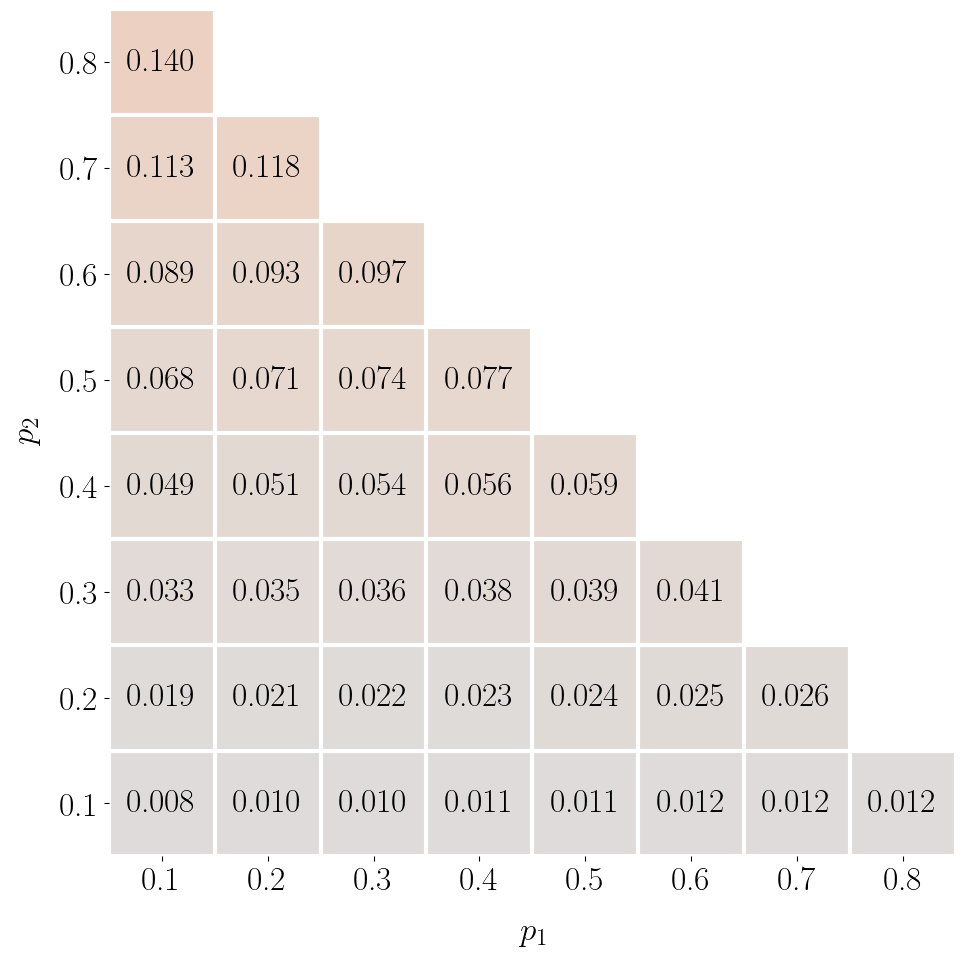
\includegraphics[width=.49\textwidth]{pics/k=200-heatmap-ndcgLoss.png}}
	\vspace{-3mm}
	\caption{Normalized exposure gain/loss and NDCG loss w.r.t. the colorblind ranking in experiment D2 (COMPAS with age as protected category) for different values of $p_1$ and $p_2$ ($k=200, \alpha=0.1$).
		%
		$p_1$ relates to group ``age 25 -- 45'', $p_2$ relates to group ``age < 25''.
		%
		Blue fields in Fig.~\ref{fig:experiments:compasAge:expGain:groupNP} -- \ref{fig:experiments:compasAge:expGain:group2} indicate that this group lost exposure w.r.t. the colorblind ranking, red fields indicate exposure gain.
	}
	\label{fig:results-moving-p}
\end{figure}

In this paper we presented the extension of \algoFAIR to multiple groups, where we guarantee ranked group fairness, without introducing a large utility loss.
%
Especially when groups largely have the same utility score in the top positions (as is the case in the COMPAS experiments) no ranking utility at all is lost in terms of NDCG or individual fairness.
%
In this case \algoFAIR only benefits the protected groups without skewing the ranking result.
%
If a protected group already receives advantageous exposure in the colorblind ranking and the ranked group fairness condition is already met via the ranking scores of the candidates, \algoFAIR preserves this.
%
A protected candidate can only lose exposure due to a protected candidate from another group being ranked up, but not due to a non-protected one.
%
Additionally the user can control the degree of fairness that is obtained in the result by setting $p_G$ to a value that is appropriate for the situation at hand.
%
This lets them transparently control the trade-off between fairness and utility, instead of having a less intuitive fairness parameter $\theta$ that operates on the barycenter of group distributions.
%
By reporting the largest utility loss and rank drop that an individual receives, we explicitly expressed trade-offs from our group fairness criterion to individual fairness as defined by~\citet{Dwork2012}. 

\spara{Future work.}
%
An important challenge is the algorithmic complexity of calculating the mTree for a particular configuration of $p_G$ and $\alpha$.
%
Though we already implemented improvements to reduce complexity, calculating an adjusted mTree of length $k=100$ with six groups takes several weeks.
%
Of course this mTree has to be calculated only once and can then be persistent and shared among users of \algoFAIR, however when a situation demands a new configuration these calculation times are currently unavoidable.
%
A significant speed-up could be achieved by programming a customized MCDF-function which can store the results of repetitive computation steps.
%
This is however very memory-intensive and the algorithm then needs to run on large computer clusters.
%
Additionally one could provide a script that fills the MCDF Cache with various configurations of $p_G$ and $\alpha$.
%
This calculation can continuously run as a separate process on a server which then provides the obtained caches to users who want to compute new mTrees.

One of the main challenges for fair ranking algorithms in general is that there is not yet much empirical evidence that re-ordering items actually helps to overcome the bias in click-probability across groups.
%
Recent research \cite{suhr2020does}, however,  suggests that guarantees for a minimum representation of underrepresented groups yield to higher selection rates in different hiring contexts, but does not mitigate user biases completely. For example if a user prefers male candidates for a moving assistance task over female candidates, ranking female candidates higher will not mitigate users' biases completely.
%
Thus, a method such as \algoFAIR may be able to increase the click probability for protected groups. Furthermore, setting the values for $p_G$ higher than desired may mitigate user biases. For example, it might be effective to set the minimum proportion for the protected group women in the context of hiring for moving assistance to $60\%$ in order to achieve a click probability of $50\%$ for this group.
%
However further research has to be conducted to study the effect on users of re-ordering items in a ranking and to understand the best means to overcome these strong prejudices against minority groups in certain domains.
%
\changed{This is an empirical question that needs to be addressed through user studies; approaches based on simulating clicks using pre-existing user preferences, such as the one used by \citet{abdollahpouri2021user}, may not uncover the actual interplay between the displayed ranking and latent user preferences.}
%
Additionally, further experimental research using synthetic data could allow us to test with a wider range of differences across groups, larger than the one that real datasets exhibit.
%
\changed{This can help us better understand the trade-offs between individual losses and increased group fairness. 
%
Our experiments show that, while decreases in NDCG are often negligible, the rank drop for an unlucky individual candidate from the non-protected group can still be large. 
%
An interesting next step for our method would be to use individual rank drops as input for a second fairness-enhancing method, that could try to optimize for individual fairness, while maintaining the ordering of groups that is required by a given mTree.}
%
Finally, robustness tests to measure the sensitivity of the rankings to noise in the qualification/score inputs could be helpful to determine to what extent they may affect our fairness objectives.

\spara{Reproducibility.}
Code and data that can be used to reproduce the experiments on this paper is available: \url{https://github.com/MilkaLichtblau/Multinomial_FA-IR}.
